\documentclass[10pt,a4paper]{article}
\usepackage[utf8]{inputenc}
\usepackage[french]{babel}
\usepackage[T1]{fontenc}
\usepackage{amsmath}
\usepackage{amsfonts}
\usepackage{amssymb}
\usepackage{hyperref}
\usepackage{graphicx}
\begin{document}

\begin{center}
{\Huge Comment ajouter ou supprimer des photos de la section 'Photos et vidéos' de ojcn.ch}
\end{center}

\section{Prérequis}
\subsection{Le logiciel FileZilla}
\subsubsection{Téléchargement de FileZilla}

\begin{enumerate}
\item Rendez-vous sur la page suivante \url{https://filezilla-project.org/download.php}
\item Cliquez sur 'Download FileZilla Client'
\item Une fois le téléchargement terminé, cliquez sur l'installateur et suivez la procédure d'installation
\end{enumerate}

\subsubsection{Configuration de FileZilla}

\begin{enumerate}
\item Ouvrez le logiciel FileZilla
\item Cliquez sur le bouton tout en haut à gauche 
\includegraphics[scale=1]{images/gestionnaire_de_sites.png} (Gestionnaire de Sites)
\item Cliquez sur 'Nouveau Site' et écrivez: photos\_public\_ojcn
\item Dans 'Hôte' entrez: ftp.ojcn.ch
\item Pour le type d'authentification choisissez 'Normale'
\item Pour l'identifiant, entrez l'identifiant fourni (par Niels)
\item Pour le Mot de passe, entre le Mot de passe fourni (par Niels)
\item Cliquez sur 'Valider'
\end{enumerate}

\section{Ajoutez et supprimer des photos}
\begin{enumerate}
\item Ouvrez le logiciel FileZilla
\item Cliquez sur la flèche vers le bas à droite du bouton 'Gestionnaire de Sites' (
\includegraphics[scale=1]{images/gestionnaire_de_sites.png})
\item Cliquez sur 'photos\_public\_ojcn' dans le menu déroulant
\item La connexion au serveur peut prendre quelques secondes, patientez
\end{enumerate}
\newpage

Une fois la connextion effectuée, l'interface se présente à peu près comme ceci: \\ 
\\
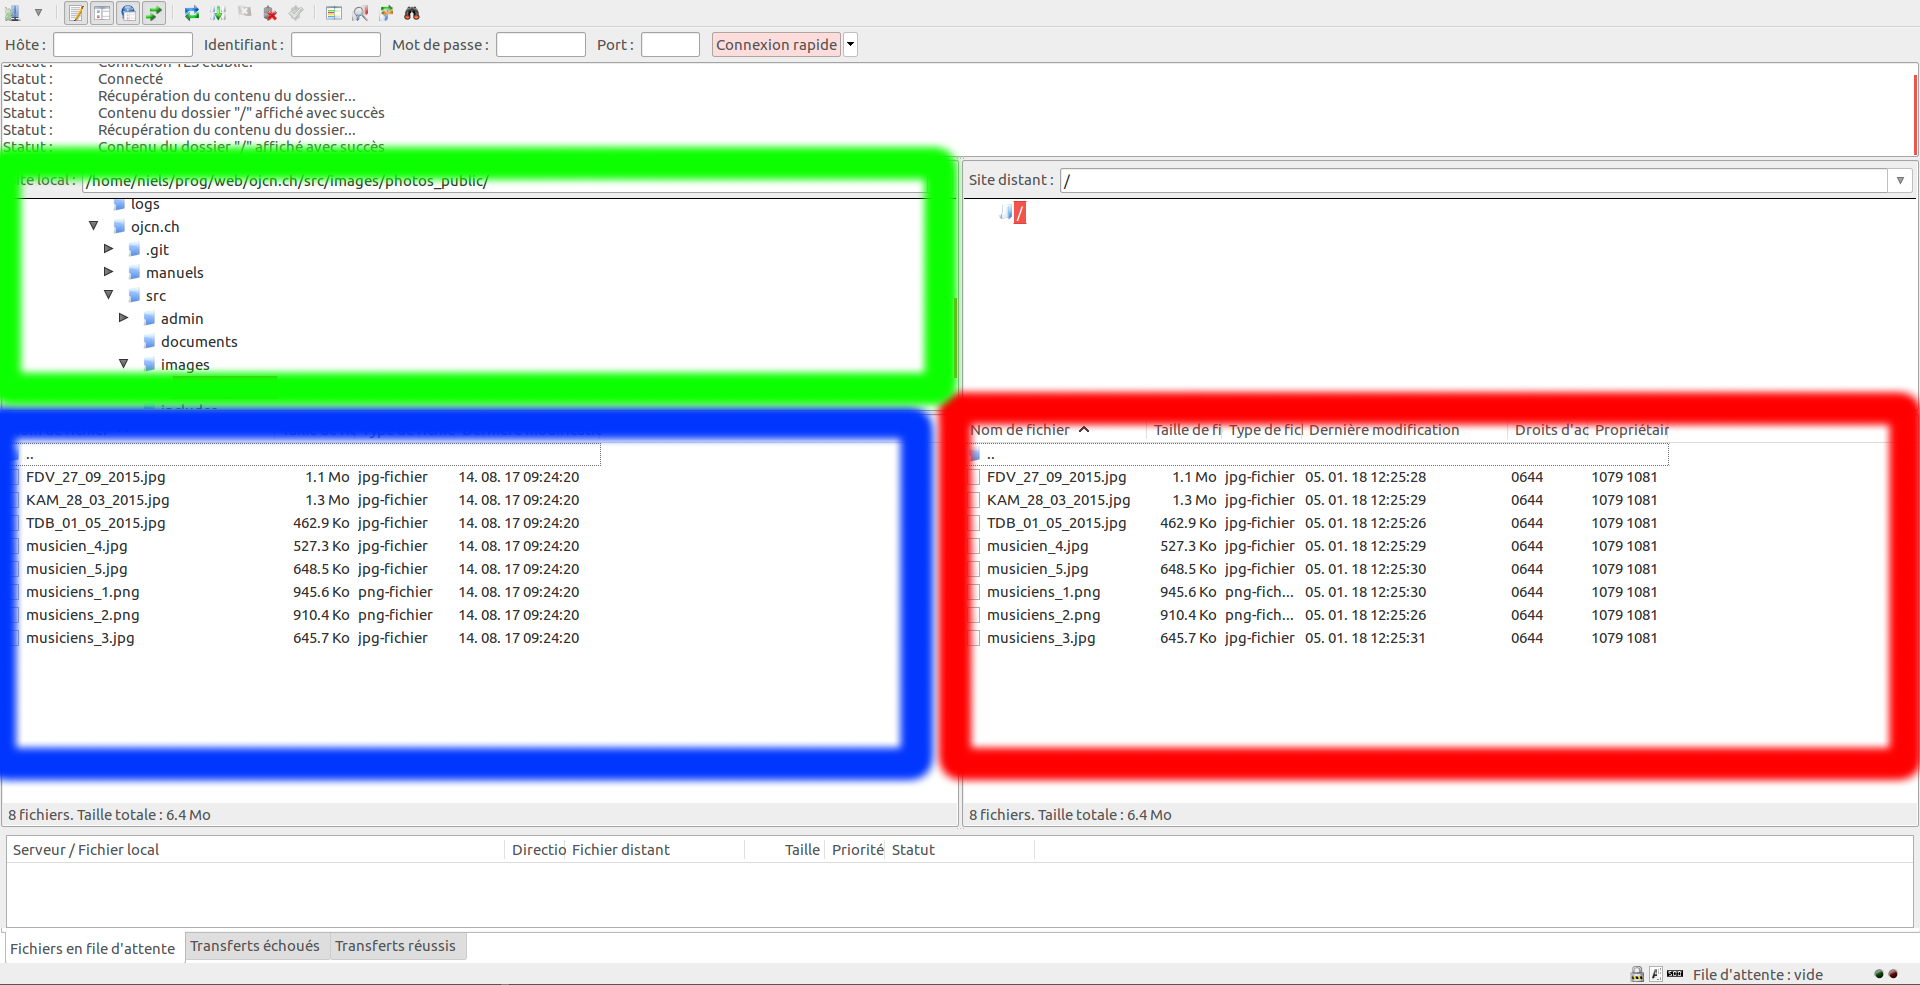
\includegraphics[scale=.2]{images/connected_modif.png} \\
\\
La zone \textbf{verte} affiche les \textbf{dossiers} de votre \textbf{disque local}.\\
La zone \textbf{bleue} représente les \textbf{fichiers} du dossier sélectionné dans la zone verte (fichiers \textbf{locaux}) \\
La zone \textbf{rouge} affiche les images du \textbf{serveur} (les images affichées sur le site) \\

\subsection{Ajouter des images sur le site}
\begin{enumerate}
\item Sélectionnez le dossier où se trouve l'image sur votre ordinateur dans la zone \textbf{verte}
\item Sélectionnez les images que vous voulez ajouter sur le site
\item Effectuez un 'glisser-déposer' depuis la zone bleue vers la zone rouge
\item Attendez que le transfert soit effectué
\end{enumerate}

\subsection{Supprimer des images du site}
\begin{enumerate}
\item Sélectionnez les images que vous voulez supprimer
\item Faites un clic droit et sélectionnez 'Supprimer'
\item Attendez quelques instants que l'opération soit effectuée
\end{enumerate}



\end{document}